\chapter{Upscaling}
\label{upscaling}

According to \cite{Lie2015}, upscaling or homogenization is defined as the process of propagating proprieties from a model with a high spatial resolution to one with a lower spatial resolution. In the case of reservoir simulation, upscaling consists of representing heterogeneous proprieties that variate inside a coarse grid block by single ,effective values for the block. Therefore, there are two models which should be considered: the coarse and the fine-grid model. For the case considered in this study, the boundaries of the coarse grid blocks will always coincide with the limit of the fine grid blocks, which means that there will be an integer number of fine grid blocks inside each of the coarse ones. Figure \ref{fig:19} illustrates the upscaling process and represents how this coarse grid will be defined.

\begin{figure}[h]
	\centering
	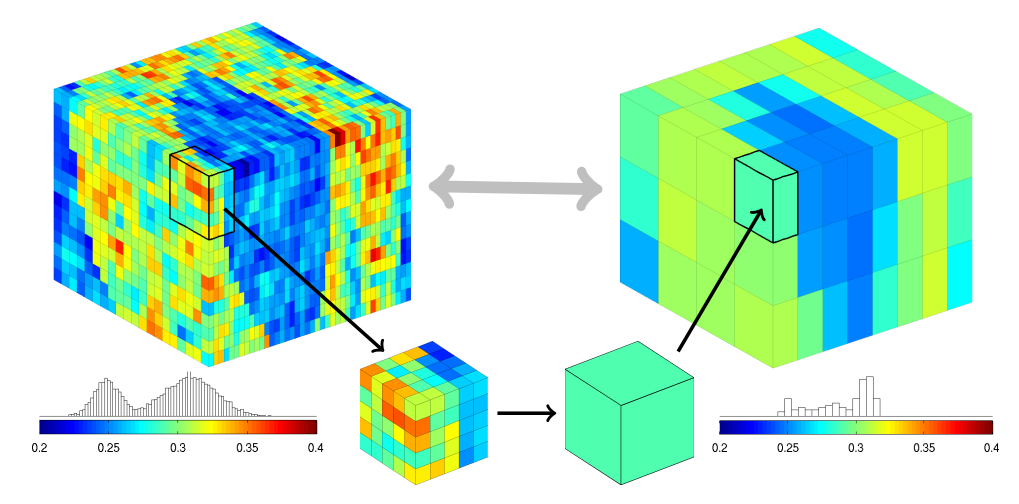
\includegraphics[width=0.8\linewidth]{Images/19}
	\caption{Illustration of porosity upscaling from a fine to a coarse grid. Source: \cite{Lie2015}.}
	\label{fig:19}
\end{figure}

\cite{Lie2015} defines two kinds of proprieties: additive and nonadditive. Additive proprieties could be upscaled by utilizing a single volumetric averaging, while nonadditive could only be averaged analytically in special cases, and the common approach is to approximate it in numerical methods. Examples of additive proprieties include porosity, net-to-gross, saturations, and concentrations; while nonadditive includes absolute permeability, relative permeability, and transmissibilities. This project is limited to the upscaling of porosity and permeability, the first being an additive and the second a non-additive propriety.

\section{Upscaling Additive Proprieties}

According to \cite{Lie2015}, porosity is the simplest example of additive propriety and could be averaged by a simple volumetric averaging. Considering $\Omega$ the region that will be upscaled, the average porosity or the porosity of the coarse grid, $\phi^{c}$ will be:
\nomenclature[G]{$\Omega$}{Region that will be upscaled}
\nomenclature[U]{$\Omega$}{Region that will be upscaled}
\nomenclature[S]{$c$}{Coarse cell}
\nomenclature[S]{$*$}{Upscaled cell}
\begin{align}
\label{Upscaling1}
\phi^{c}=\frac{1}{\Omega}\int_{\Omega}\phi(x,y,z)dV.
\end{align}
\noindent
The $c$ index will be consistently utilized to represent an upscaled value, which is the effective, representative value for the coarse grid blocks. Other additive proprieties can be upscaled in a similar form, except that their bulk average should be weighted with porosity. Considering $a$ an additive propriety other than porosity:

\begin{align}
\label{Upscaling3}
a^c=\left[\int_{\Omega}\phi(x,y,z)dV\right]^{-1}\int_{\Omega}a(x,y,z)\phi(x,y,z)dV.
\end{align}

%Wagner{Coloque uma lista de todas as propriedades a(x,y,z) que serão upscaladas segundo propriedades aditivivas.}

\section{Upscaling Absolute Permeability}

\cite{Lie2015} divides upscaling into two distinct segments: single-phase and multiphase. The propriety scaled up in single-phase upscaling is the absolute permeability, while in multiphase upscaling it is the relative permeability. Since this project does not comprises a multiphase flow scenario, the only permeability to be averaged will be the absolute one. Since it is a nonadditive propriety, it is not possible to utilize a simple volumetric averaging. \cite{Lie2015} explains the process of absolute permeability upscaling by utilizing the flow described by the Poison equation:
\nomenclature[R]{$K$}{Permeability tensor}
\begin{align}
\label{Upscaling4}
\nabla \cdot K \nabla p = 0.
\end{align}
\noindent
where $K$ is the permeability tensor. The majority of upscaling techniques consists in determining an effective permeability tensor $K^c$ that reproduces in the coarse grid blocks the flow rate inside it, in the fine-scale region. Mathematically:

\begin{align}
\label{Upscaling5}
\int_{\Omega}K(x,y,z)\nabla p dV=K^c \int_{\Omega}\nabla p dV.
\end{align}
\noindent
Eq. \ref{Upscaling5} states that the net flow rate $v_\Omega$ through $\Omega$ is associated with the average pressure gradient $\nabla_\Omega p$ in $\Omega$ by the upscaled Darcy's law, which its tensorial form is:

\begin{align}
\label{Upscaling6}
v_\Omega=-K^c\nabla_\Omega p.
\end{align}
\noindent
\cite{Lie2015} states that the permeability tensor is not uniquely defined by Eq. \ref{Upscaling5} for a pressure field $p$, in other words, there is not a unique $K^c$ tensor that accounts for any $p$. Thus, $K^c$ depends on the flow through $\Omega$, which is determined by the boundary conditions in the fine-scale region. \cite{Lie2015} also states that if those boundary conditions are exactly known, it is possible to compute the true effective permeability. However, one could not know exactly what those boundary conditions are unless the problem is already solved. Therefore, what is generally done is performing a reasonable and representative guess giving fairly accurate results for several flow scenarios.

\subsection{Flow-based Methods}

\cite{Lie2015} states that flow-based upscaling consists of imposing boundary conditions around each coarse block and solve the Eq. \ref{Upscaling4} to determine fine-scale pressure and flow rates and utilize those for defining net flow rates and average pressure gradients, which could be inverted to determine $K^c$ from Eq. \ref{Upscaling6}. According to \cite{Nunna2015}, the industry has been focused on developing upscaling algorithms based on permanent, incompressible flow. This project approaches upscaling by utilizing the averaging techniques, which besides being simple, are foreseen to give a more accurate representation than the flow-based methods.

\subsection{Averaging Methods}

According to \cite{Lie2015}, averaging methods for upscaling consist of utilizing analytical averaging, most of the times following the power average formula:
\nomenclature[R]{$A_p$}{Generic average operator utilizing the power average notation}
\nomenclature[R]{$A_1$}{Arithmetic average operator}
\begin{align}
\label{Upscaling7}
K^c=A_p(K)=\left(\frac{1}{|\Omega|}\int_{\Omega}K(x,y,z)^pdV\right)^{\frac{1}{p}},
\end{align}
where $p=1$ and $p=-1$ respectively refer to the arithmetic and harmonic means, and $p \rightarrow 0$ corresponds to the geometric mean. According to \cite{Wiener1912}, for a statistic homogeneous medium, the correct upscaled permeability is bounded above and below by the arithmetic and harmonic means, respectively. For a steady-state the Eq. \ref{Upscaling6} is:
\begin{align}
\label{Upscaling8}
\frac{\partial}{\partial t}v_\Omega= 0,
\end{align}
\begin{align}
\label{Upscaling9}
\frac{\partial}{\partial t} \left(-K^c\nabla_\Omega p\right)= 0.
\end{align}
Considering a permanent permeability tensor:
\begin{align}
\label{Upscaling10}
-K\frac{\partial}{\partial t} \left(^c\nabla_\Omega p\right)= 0.
\end{align}
Considering a system of layers with homogeneous permeability values in perpendicular to the pressure gradient, as illustrated in Figure \ref{fig:20}:

\begin{figure}
	\centering
	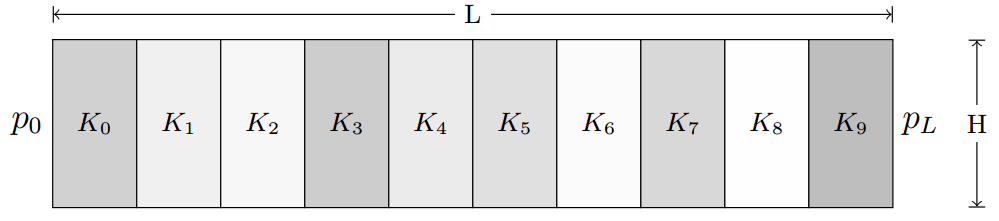
\includegraphics[width=0.7\linewidth]{Images/20}
	\caption{Illustration of a perfectly stratified medium with layers perpendicular to the pressure gradient. According to \cite{Lie2015}, in this setting harmonic is the appropriate averaging for upscaling permeability. Source: \cite{Lie2015}.}
	\label{fig:20}
\end{figure}
\noindent
It is possible to write:
\begin{align}
\label{Upscaling11}
K*\int_{0}^{L}\frac{dp(x)}{dx}dx=K^c(p_L-p_0).
\end{align}
Moreover, from Eq. \ref{Upscaling8}:
\begin{align}
\label{Upscaling12}
\int_{0}^{L}K(x)\frac{dp(x)}{dx}dx= \int_{0}^{L}v dx = -Lv.
\end{align}
Applying Eqs. \ref{Upscaling11} and \ref{Upscaling12} in Eq. \ref{Upscaling5}:
\begin{align}
\label{Upscaling13}
v=-K^c\frac{(p_L-p^0)}{L}.
\end{align}
From Darcy's law, Eq. \ref{Upscaling10}:
\begin{align}
\label{Upscaling14}
\int_{0}^{L}\frac{dp}{dx}(x)dx=-\int_{0}^{L}\frac{v}{K(x)}dx,
\end{align}
\begin{align}
\label{Upscaling15}
\int_{0}^{L}\frac{dp}{dx}(x)dx=K^c\frac{(p_L-p^0)}{L}\int_{0}^{L}\frac{1}{K(x)}dx,
\end{align}
\begin{align}
\label{Upscaling16}
\int_{0}^{L}\frac{dp}{dx}(x)dx=K^c\left(\int_{0}^{L}p(x)dx\right)\frac{1}{L}\int_{0}^{L}\frac{1}{K(x)}dx,
\end{align}
Hence:
\begin{align}
\label{Upscaling17}
K^c=A_{-1}(K)=\left(\frac{1}{L}\int_{0}^{L}\frac{1}{K(x)}dx\right)^{-1},
\end{align}
which shows that harmonic is the correct way to upscale permeability in such a scenario. On the other hand, for a system of homogeneous permeabilities values parallel to the pressure gradient, according to Figure \ref{fig:21}. Since the permeability, in this case, is constant along the direction $x$, the pressure could be described as:
\begin{align}
\label{Upscaling21}
p(x,y)=p_0+\frac{x(p_L-p_0)}{L}.
\end{align}
Moreover, it is possible to write:
\begin{figure}
	\centering
	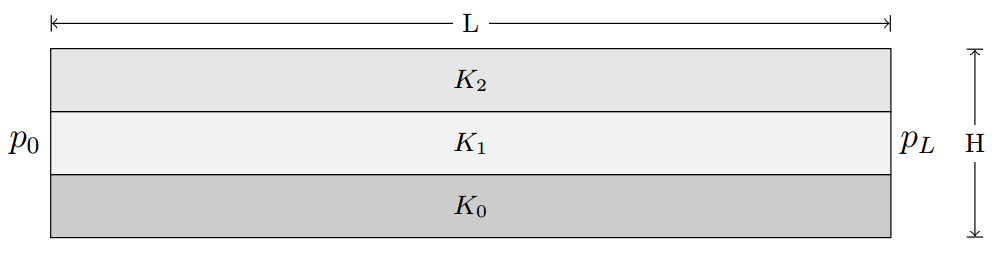
\includegraphics[width=0.7\linewidth]{Images/21}
	\caption{Illustration of a perfectly stratified medium with layers parallel to the pressure gradient. According to \cite{Lie2015}, in this setting arithmetic is the appropriate averaging for upscaling permeability. Source: \cite{Lie2015}.}
	\label{fig:21}
\end{figure}
\begin{align}
\label{Upscaling18}
K^c\int_{0}^{H}\int_{0}^{L}\frac{\partial p(x,y)}{\partial x}dx dy=K^cH(p_L-p_0)
\end{align}
and
\begin{align}
\label{Upscaling19}
\int_{0}^{H}\int_{0}^{L}K(x,y)\frac{\partial p(x,y)}{\partial x}dx dy=\frac{p_L-p_0}{L}\int_{0}^{H}\int_{0}^{L}K(x,y)dx dy.
\end{align}
Applying Eqs. \ref{Upscaling18} and \ref{Upscaling19} in Eq. \ref{Upscaling5}:
\nomenclature[R]{$H$}{Total height in a reservoir}
\begin{align}
\label{Upscaling20}
K^c=A_1(K)=\frac{1}{HL}\int_{0}^{H}\int_{0}^{L}K(x,y)dx dy,
\end{align}
which is arithmetic averaging. By those two methods, it is possible to create a permeability tensor for scenarios like the described in the Figures \ref{fig:20} and \ref{fig:21}:
\begin{equation}
K^c=
\begin{bmatrix}
A^x_{-1}(K)	&0\\
0	&A^x_{1}(K)
\end{bmatrix}
\end{equation}
and
\begin{equation}
K^c=
\begin{bmatrix}
A^y_{1}(K)	&0\\
0	&A^y_{-1}(K)
\end{bmatrix}
\end{equation}
where the superscripts x and y in the averaging operator $A$ means that it is only applied in that direction. For modeling flow in more directions and also for less idealized heterogeneous regions, it is possible to combine those two methods through the tensor:
\begin{equation}
\label{arithmeticharmonic}
K^c=
\begin{bmatrix}
A^{yz}_{1}(A^{x}_{-1}(K))	&0	&0\\
0	&A^{xz}_{1}(A^{y}_{-1}(K))	&0\\
0	&0	&A^{xy}_{1}(A^{z}_{-1}(K))
\end{bmatrix}
\end{equation}
This method is called the harmonic-arithmetic averaging and, according to \cite{Lie2015}, might give a fair upscaling in layered reservoirs when the main direction of flow is along with the layers. This method provides a tight lower bond on permeability, while its inverse, the arithmetic-harmonic averaging, provides a tight upper bound.

